\documentclass[../Assignment-3-LPSMT.tex]{subfiles}
\graphicspath{{\subfix{../img/}}}

\begin{document}

\chapter{Implementazione}

Manga-check è stata sviluppata seguendo un modello a singola Activity che naviga tra vari Fragment$\dots$.\\

\section{Uso degli XML}

L'idea originale era di implementare un sistema di log in facoltativo per gli tutti gli utenti che volevano mantenere sincronizzata la propria reading list.\\
Dopo una revisione con il docente abbiamo però optato per una soluzione dall'implementazione più rapida, ovvero un importa/esporta manuale.\\
Abbiamo deciso di adottare come standard dei file salvati in locale \emph{xml}, la scelta è stata fatta per la semplicità nella verifica manuale dei dati, avendo fatto fatto largo uso della shell abd risultava molto facile verificare se il file era stato scritto in modo corretto.\\
La modificata e la gestione semplice dei file è stat possibile grazie al package \href{https://kotlinlang.org/api/latest/jvm/stdlib/org.w3c.dom/}{org.w3c.dom}, un wrapper di javascript per la gestione di elementi del DOM, che ci ha permesso di getsire ogni entry dei file \emph{xml} come un nodo con al suo interno degli attributi identificati dal nome dei campi.

\begin{center}
  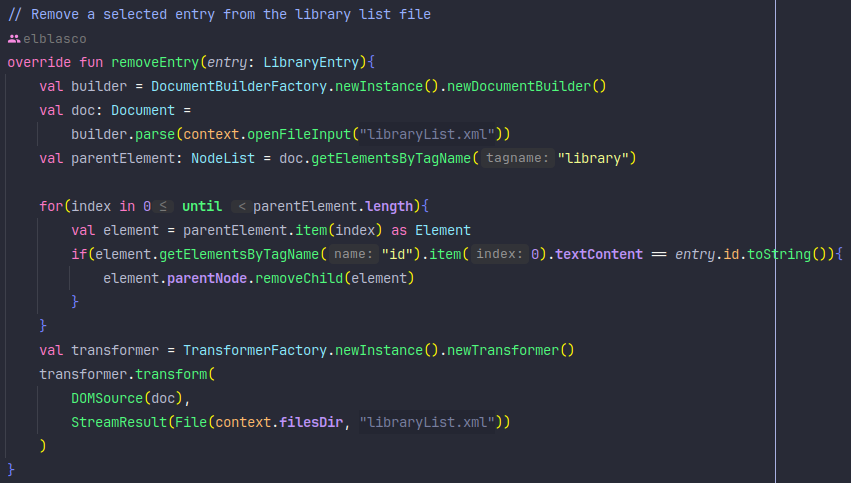
\includegraphics[scale=0.5]{removeEntry_XML.png}
  \captionof{figure}{Rimozione di una entry nella library list}
\end{center}

\section{Richieste API}

Le richieste API sono state getsite con il sopracitato package \emph{ktor}, una parte della formattazione delle rispose alle API è stata getsita lato server per ridurre il codice da scrivere nell'applicazione e non sprecare rallentare troppo l'app.\\
Per getsire le risposte al meglio abbiamo di deciso di gestire lato client come delle matrici di stringhe.\\
Nel caso sottostante riceviamo i dati come una stringa che poi viene separata grazie ad una regex ed in seguito inserita in una matrice $[n][2]$ in cui $[n][0]$ contiene l'id del manga richiesto mentre $[n][1]$ il nome.

\begin{center}
  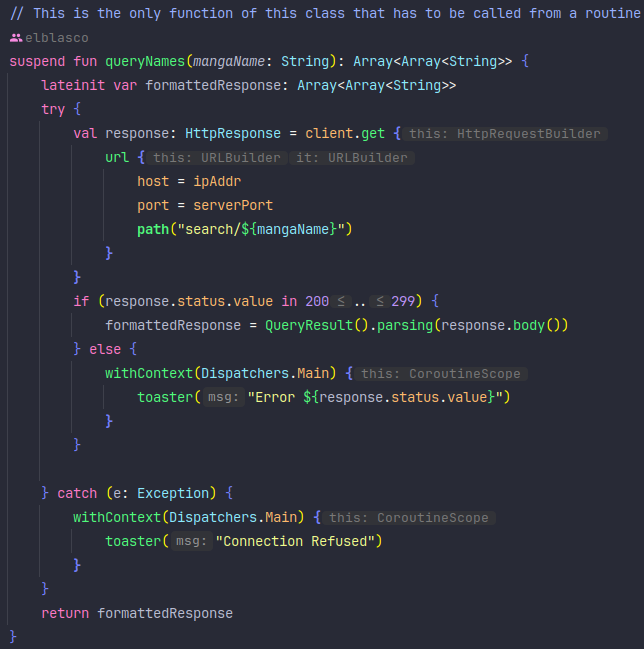
\includegraphics[scale=0.5]{queryNames.png}
  \captionof{figure}{Query dei vari nomi possibili per il manga}
\end{center}

\section{Uso di Safe Args}

Nel progetto abbiamo dovuto trasferire alcuni dati tra due fragment, come indicato nella documentazione Android abbiamo deciso di usare il \emph{navigation graph}, quindi vincolando i dati ad avere un determinato tipo.\\
Questo vincolo è stato posssibile grazie all'utilizzo del plug in \href{https://developer.android.com/guide/navigation/use-graph/pass-data#Safe-args}{Safe Args} che ci ha permesso di specificare delle \emph{action} con un paylod di dati tipizzati.\\
Come descritto nelle linee guida non abbiamo passato in questi payload strutture complesse, ma solo dati di tipi primitivi come \emph{Int} e \emph{String}.

\begin{center}
  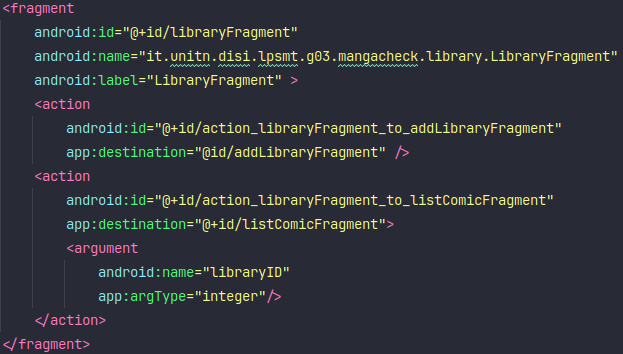
\includegraphics[scale=0.5]{action_navgraph.png}
  \captionof{figure}{Esempio di action con Safe Args}
\end{center}

\section{Backup \& Cache}

\end{document}
